\documentclass[11pt]{article}
\usepackage[spanish]{babel}
\decimalpoint
\usepackage[utf8x]{inputenc}
\usepackage{amsfonts}
\usepackage{MnSymbol}
\usepackage{graphicx}
\usepackage{float}
\usepackage{wasysym}
\usepackage{pdfpages}
\usepackage[margin=0.5in,left=1in,right=1in, bottom = 1in, includehead]{geometry}
\usepackage{amsmath}
\usepackage{multicol}
\usepackage{caption}
\usepackage{subcaption}
\renewcommand{\baselinestretch}{1.3}


%% NEW Commands
\newcommand{\klein}{\text{*}}  
\newcommand{\R}{\mathbb{R}}
\newcommand{\N}{\mathbb{N}}

\newcommand{\red}[1]{\textcolor{red}{#1}}
\newcommand{\blue}[1]{\textcolor{blue}{#1}}
\newcommand{\green}[1]{\textcolor{green}{#1}}


\title{Reporte semanal: Agosto 11-17}
\author{Jorge Ballote}
\begin{document}

% \includepdf[pages=1]{portada_proyecto_02.pdf}
\maketitle
% ---- 1. INTRODUCCIÓN -----------------------------------------
\section{Introducción} Ya que se realizarán reportes semanales, el algorítmo básico se toma por entendido, y por consiguiente sólo se mencionan los cambios realizados al algoritmo inicial.

% ---- 2. Objetivos de la semana -----------------------------------------
\section{Objetivos de la semana}
Esta semana fue destinada a lo siguiente.
\begin{enumerate}
    \item Celdas o píxeles, con proporción  entre “wins and losses”.
    \item Utilizar diferentes proporciones en las celdas (“wins vs total”, “loss vs total”)
    \item En cada celda hacer agregar el retorno del trace (en vez de +1, -1).
\end{enumerate}
Los objetivos fueron cumplidos en tiempo. En las siguiente secciones, se analizan los resultados obtenidos.

% ---- 3. ALGORITMOS -----------------------------------------
\section{Modificaciones al algoritmo}
El Método de entrenamiento de una Grid, se describe en el reporte anterior y en el artículo [1]. Tal como se menciona en los objetivos, realizamos 3 modificaciones independientes.

\subsection{Proporción entre 'Wins' y 'Losses'}
En el algoritmo original, cuando una trace ganadora pasaba por una celda, a esa celda se le añadía un +1. En caso contrario, se añadía -1. En esta nueva versión, cada celda tiene un registro de $[W,L]$ donde $W$ es la cantidad de traces ganadoras que pasaron por esa celda y $L$ la cantidad de traces perdedoras que pasaron por esa celda.

De modo que es posible encontrar la proporción $W/L$ (En el algoritmo original es $W-L$). Sin embargo, puede ocurrir que en alguna celda $L=0$, lo cuál genera un error de división entre cero. Una manera de solucionar esto es agregar $\epsilon >0$ a $W$ y a $L$ en cada celda. De modo que se tendría la división
\begin{equation}
    \frac{W + \epsilon}{L + \epsilon}
\end{equation}
Hay que ser cuidadosos con la selección de $\epsilon$, pues si se escoge muy grande, los valores $W$ y $L$ se vuelven irrelevantes, y todas nuestras fracciones serían aproximadamente 1. Pero si  se selecciona muy pequeño, corremos el riesgo de que celdas cuyos valores sean demasiado elevados, logrando que la media sea menos significativa. En la práctica, se obtivieron resultados muy buenos usando $\epsilon=100$ o $\epsilon=1000$. Sin embargo, hablaremos más al respecto de este hiperparámetro en la sección de resultados.

\subsection{Diferentes proporciones.}
A pesar de que el artículo [1] menciona la proporción $W/L$. Una de las preguntas naturales, es ¿Qué ocurriría si en vez, utilizo $W/T$. Dónde el total $T$ es $T = W+L$. 

Otras posibles proporciones son
\begin{itemize}
    \item $T/L$: Cabe aclarar que $L/T$ no es una buena proporción, debido a que las celdas con mayor puntaje serían aquellas con mayor cantidad de derrotas. Por otro lado $\frac{T}{L} = \frac{W+L}{L} = 1 + \frac{W}{L}$, por lo que no hay gran diferencia con la proporción $W/L$. Sin embargo, también fue implementada.
    \item $(WL + T^2)/(2TL)$: Aunque parece una división sin sentido, en realidad es igual a $\frac{1}{2}\left(\frac{W}{T} + \frac{T}{L}\right)$.
\end{itemize}
Ya que también, es un entrenamiento de grid basados en proporción, también es necesario el uso de un factor $\epsilon > 0$.

\subsection{Agregar el retorno del trace}
En el algoritmo original, cada trace sólo se toma como ganador o perdedor, sin importar cuánto ganó o perdió. Por tanto, en esta modificación cada celda conserva los valores $[\hat W, \hat L]$ dónde $\hat W$ es la suma de los porcentajes ganados por las traces que pasaron por esa celda. y $\hat L$ es el análogo, pero con pérdidas.

En este mismo esquema, es posible calcular el valor de la celda usando $\hat W - \hat L$, o aplicando las proporciones descritas en la modificación anterior.

\section{Metodología}
Sin importar que estilo de Grid se utilice, siempre se evalúa un trace en esta grid, y se obtiene una puntuación. Se esperaría que las traces con puntuaciones bajas fuesen perdedoras y que las traces con puntuaciones altas fuese ganadoras. ¿Cómo determinamos si una puntuación es alta o baja? Lo que haremos será definir 2 umbrales. Un umbral superior $T^+ = \mu + alpha^+\sigma$ y un umbral inferior $T^- = \mu - alpha^-\sigma$. Si las puntuaciones superan el umbral superior, serán consideradas puntuaciones altas, y si las puntuaciones están por debajo del umbral inferior, serán consideradas puntuaciones bajas.

Por el momento, se hicieron experimentos con 4 distintas parejas de umbrales.
\begin{enumerate}
    \item $\alpha^+ = \alpha^- = 0.4$
    \item $\alpha^+ = \alpha^- = 0.8$
    \item $\alpha^+ = \alpha^- = 0.12$
    \item $\alpha^+ = \alpha^- = 0.16$
\end{enumerate}
Donde $\mu$ y $\sigma$ representan la media y la desviación estandar de las puntuaciones del conjunto de entrenamiento, respectivamente. 

Para la presentación de resultados, usaremos 2 formas de evaluar nuestro algoritmo. 
\begin{enumerate}
    \item \textbf{Desempeño en los últimos días:} Simplemente, ¿Si hubiésemos usado nuestro algoritmo en los últimos $d$ días, ¿Cuántas veces hubiésemos acertado?
    %\item \textbf{Desempeño en los últimos días por intervalos:} Dividimos el conjunto de datos entero, en $p$ intervalos. Se hacen $p$ experimentos difentes. El $i$-ésimo experimento es juntando los primeros $i$ intervalos, y evaluando el desempeño en los últimos $n$ días. Luego, se hace un promedio de los desempeños de todos los experimentos realizados.
\end{enumerate}

%Nótese que el \textbf{Desempeño en los últimos días} es el equivalente al Desempeño en los últimos días por Intervalos con $p=1$.


\subsection{Desempeño en los últimos días}
Para poder, determinar el desempeño de una grid en los últimos $n$ días es necesario entrenar $n$ grids diferentes, y calcular las medias y las desviaciones estandar de las scores del conjunto de entrenamiento. Es posible prescindir de entrenar $n$ grids diferentes, entrenando únicamente vez la grid y actualizando la matriz $n$. Sin embargo, el cálculo de las medias y desviaciones estandar sigue siendo un proceso muy costoso. Por buena suerte para nosotros, las medias y las desviaciones estandar no cambian mucho después de añadir nuevas traces a la grid. 
\begin{figure}[H]
    \centering
    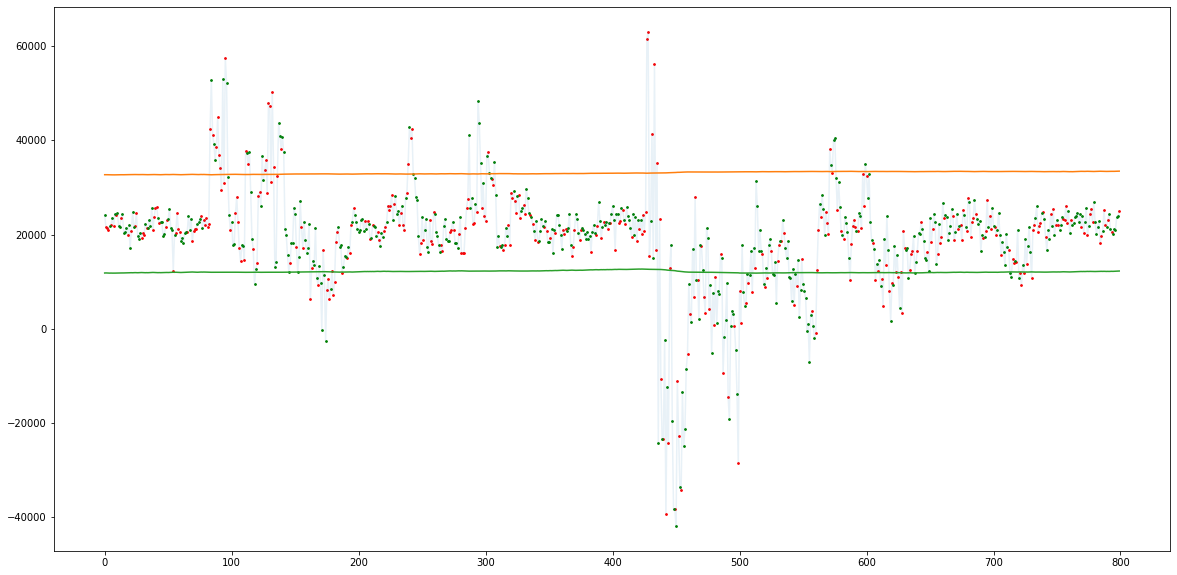
\includegraphics[width=4.5in]{../../src/imgs/std_variable800.png}
    \caption{Puntuaciones de los últimos 800 días. Los puntos verdes, son días ganadores, y los puntos rojos días perdedores. Las curvas superior e inferior representan $T^+$ y $T^-$. Nótese que son casi líneas rectas.}
\end{figure}
Por lo que en vez de actualizar los valores estadísticos, usaremos la media y la desviación estandar de la primera grid entrenada, y usaremos esos valores para determinar los umbrales en el resto de los días.


Las métricas a consideran serán las siguientes:
\begin{enumerate}
    \item \textbf{Accuracy:} Predicciones correctas, entre total de predicciones
    \item \textbf{Accuracy por encima del umbral:} Accuracy, tomando en cuenta únicamente el sample de puntuaciones por encima de $T^+$
    \item \textbf{Accuracy por debajo del umbral:} Accuracy, tomando en cuenta únicamente el sample de puntuaciones por debajo de $T^-$
    \item \textbf{Participation:} Porcentaje de participación. Es decir total de predicciones, entre el total de datos de prueba.
    \item \textbf{Participation por debajo del umbral:} Participación, tomando en cuenta únicamente el sample de puntuaciones por debajo de $T^-$
    \item \textbf{Participation por debajo del umbral:} Participación, tomando en cuenta únicamente el sample de puntuaciones por debajo de $T^-$
\end{enumerate}
\

\section{Resultados}
A continuación presentamos del desempeño en los últimos 365 días de diferentes grids. Por el momento, usaremos únicamente grids cuadradas de $M\times M$. Las granularidades que usaremos son $M = 15, 30, 60$. y usaremos traceSize = $M$. Los tipos de grid a probar son 'wins' y 'earnings'. y las operaciones son 4: $W-L$ (El default), $W/L$, $W/T$, $T/L$. Y considerando que usaremos 4 diferentes valores de umrales, obtenemos un total de $3\times2\times 4\times 4 = 96$ experimentos diferentes.

Aquí presentamos los 5 mejores experimentos. Pero en el proyecto se anexa un archivo .csv con la información completa.

\begin{tabular}{llrrrr}
\hline
{} &                       parameters &   accuracy &  participation &  acc\_above &  acc\_below \\
\hline
28 &      (15,15,15,1.6,1.6,T/L,wins) &  59.016393 &      16.712329 &  73.333333 &  54.347826 \\
24 &      (15,15,15,1.6,1.6,W/L,wins) &  59.016393 &      16.712329 &  73.333333 &  54.347826 \\
20 &      (15,15,15,1.2,1.2,T/L,wins) &  58.823529 &      23.287671 &  75.000000 &  52.459016 \\
16 &      (15,15,15,1.2,1.2,W/L,wins) &  58.823529 &      23.287671 &  75.000000 &  52.459016 \\
45 &  (30,30,30,0.8,0.8,T/L,earnings) &  57.142857 &       9.589041 &  61.111111 &  52.941176 \\
\hline
\end{tabular}

El desempeño en los últimos años no siempre asegura un rendimiento futuro. Sin embargo, si se hubiese utilizado este algoritmo  con los 
En el último año, el mercado ha tenido el $58.79\%$ de días ganadores. Por lo que la accuracy total general, no es demasiado superior. Sin embargo, tomando únicamente señales de compra, se pueden obtener resultados de $73 \%$.  

\section{Conclusiones}

Usando los parámetros parámetros (15,15,15,1.2,1.2,T/L,wins) hubiésemos acertado un $75\%$ de las veces, por lo que los resultados parecen prometedores en ese sentido. Por otro lado, parece que las grids y traces pequeñas benefician al algoritmo, pues los experimentos con grids de $15\times 15$ están todos en la primera mitad de la tabla. tal cómo se esperaba, las proporción $W/L$  es equivalente a $T/L$. Un caso destacable, es el experimento de la columna 28 en el documento csv. Pues tiene un $66\%$ de acc$\_$above, pero con una participación del $21\%$! Ya que el porcentaje de participación con buenos resultados, ronda siempre por debajo del $10\%$.  Por el momento no es claro si los gipos de grid tengan influencia en los resultados, pero parece que el uso de proporciones mejora ligeramente el rendimiento. Es recomendable \textbf{no} comenzar a invertir,  hasta tener el reporte final de resultados.

\end{document}
